\documentclass[]{article}

%%% Работа с русским языком
\usepackage{cmap}					% поиск в PDF
\usepackage{mathtext} 				% русские буквы в фомулах
\usepackage[T2A]{fontenc}			% кодировка
\usepackage[utf8]{inputenc}			% кодировка исходного текста
\usepackage[english,russian]{babel}	% локализация и переносы


%%% Дополнительная работа с математикой
\usepackage{amsmath,amsfonts,amssymb,amsthm,mathtools} % AMS
\usepackage{icomma} % "Умная" запятая: $0,2$ --- число, $0, 2$ --- перечисление

%% Номера формул
%\mathtoolsset{showonlyrefs=true} % Показывать номера только у тех формул, на которые есть \eqref{} в тексте.
%\usepackage{leqno} % Немуреация формул слева


\usepackage{hyperref}
\usepackage[usenames,dvipsnames,svgnames,table,rgb]{xcolor}
\hypersetup{				% Гиперссылки
    unicode=true,           % русские буквы в раздела PDF
    pdftitle={Заголовок},   % Заголовок
    pdfauthor={Автор},      % Автор
    pdfsubject={Тема},      % Тема
    pdfcreator={Создатель}, % Создатель
    pdfproducer={Производитель}, % Производитель
    pdfkeywords={keyword1} {key2} {key3}, % Ключевые слова
    colorlinks=true,       	% false: ссылки в рамках; true: цветные ссылки
    linkcolor=red,          % внутренние ссылки
    citecolor=black,        % на библиографию
    filecolor=magenta,      % на файлы
    urlcolor=cyan           % на URL
}

\usepackage{csquotes} % Инструменты для ссылок

\usepackage[backend=biber,bibencoding=utf8,sorting=ynt,maxcitenames=2,style=authoryear]{biblatex}


\title{Задачи по алгоритмической теории игр}
\newcommand{\task}[1]{\textbf{Задача #1. }}

\bibliography{bib}
\addbibresource{../essay/sample.bib}

\begin{document}
\maketitle

\task{1}
Рассмотрим задачу о справедливом дележе для $N$ агентов.

\textbf{Вопрос 1.} Какое максимальное количество пар завидующих агентов может быть при пропорциональном дележе? (Если зависть взаимная, то пара считается дважды).

\textbf{Указание.} доказать, что при пропорциональном дележе участник не может завидовать всем остальным. Можно ли сделать так, чтобы он завидовал почти всем? Будут ли участники влиять друг на друга?

Что такое задача о справедливом дележе? \cite{gm}

\begin{itemize}
\item $N$ участников, 1 шоколадка
\item Разным участникам нравятся разные части шоколадки 
\item Как поделить по-честному?
\end{itemize}

\textbf{Определение 1.} Пропорциональный дележ --- дележ, при котором каждый считает, что получил не меньше $1/N$. 
\textbf{Определение 2.} Дележ без зависти --- когда каждый считает, что его кусочек лучше, чем кусочек любого другого.

\textbf{Ответ 1.} При пропорциональном дележе участник не может завидовать всем остальным, потому что уже на первом шаге он получает не меньше половины шоколадки, а последующие дробления производит на совершенно равнозначные (с его точки зрения) части.

\textbf{Ответ 2.} После первого дележа второй игрок может начать иметь смещенные представления о ценности (с точки зрения первого игрока), или вдруг стать альтруистом, и оставить себе очень малое количество шоколадки, тогда первый останется с не менее чем $1/4$ (но не сильно больше), а третий игрок останется с почти $1/4$ и почти половиной. Тогда первый будет завидовать третьему, а второй не будет завидовать никому (потому что поделил справедливо со своей точки зрения).

В случае с тремя завидовать может только один (невозможно, чтобы оба других получили больше, чем он, ведь он отдаст ровно половину, а у двух других останется либо поровну с его точки зрения, либо у одного больше).

А вот что будет происходить при произвольном $N\in\mathbb{N}$?

Пусть $\Omega$ --- цельное благо.
Для каждого игрока рассмотрим функцию полезности $u_n: 2^\Omega \to \mathbb{R}$.
То есть можно сказать, как оценивается любое из подмножеств $\Omega$ для игрока $n$.
Ясно, что $2^\Omega$ будет алгеброй.

И когда алгоритм закончит работу, нужно будет просто сравнить для каждого игрока $n$ $u_n(Profit_n)$ и $u_n(Profit_{n^{-1}})$.

%%%%%%%%%%%%%%%%%%%%%%%%%%%%%%%%%%%%%%%%%%%%%%%%%%%%%%%%%%%%%%%%%%%%%%%%%%%%%%%%%%%%%%%%%%%%%%%%%%%%%%%%%%%%%%%%%

\task{2} Придумайте задачу о маршрутизации делимого трафика, в которой цена анархии равна в точности  $1.2$.

\textbf{Указание:} модифицировать цифры в одной из стандартных конструкций (пример Пигу или парадокс Браесса).

\textbf{Definition. } The \textit{price of anarchy} of a game is the ratio between the worst objective function (целевая функция) value of an equilibrium of the game and that of an optimal outcome}

%%%%%%%%%%%%%%
\begin{comment}
\textbf{Задача о маршрутизации делимого трафика}\cite{t2014}

Дан ориентированный граф $G=(V,E)$ без петель и кратных ребер. Дан некоторый набор троек $(s_i, t_i, x_i)$, где $s_i,t_i\in V, x_i>0, i=\overline{1,n}$. 
Также для каждого ребра $e\in E$ задана неубывающая функция $c_e(y)$, т.ч. $c_e(0)\ge0$. 

Потоком по сети называется набор неотрицательных чисел ${x_{ie}}_{i=1,...,n, e\in E}$.

Потоком через вершину называется $f_{iv}=\Sigma_{e выходит из v}x_{ie} - \Sigma_{e входит в v}x_{ie}$. Поток называется допустимым, если $\forall i f_{is_i}=x_i, f_{it_i}=-x_i, f_iv=0$ при $v\ne s_i,t_i$. Издержками от потока называется величина $\Sigma_e c_e (\Sigma_i x_{ie})$. 
\end{comment}
%%%%%%%%%%%%

\textbf{Пример Пигу (Pigou`s Example)} \cite[447]{agt}

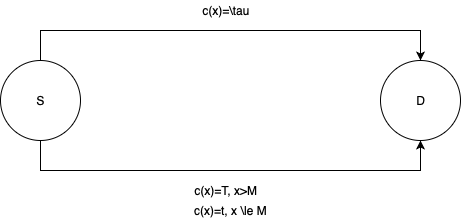
\includegraphics{pigou}

Two disjoing edges connect source vertex $s$ to a destination vertex $t$. Each edge has a \textit{cost function} $c(\dot)$, which describes the cost (e.g., travel time) incurred by users of the edge, as a function of the amount of traffic routed on the edge. We are interested in the price of anarchy\cite{poa} of this game.

Suppose one unit of traffic, representing a very large population of players, and each player chooses independently between the two routes from $s$ to $t$. Assuming that each player aims to minimize its cost, the lower edge is a dominant strategy. 
In the unique equilibrium, all of them incure one unit of cost. 

Optimal outcome is to minimize average cost for players.



\printbibliography

\end{document}
